\documentclass[11pt]{article}
\usepackage{graphicx}
\usepackage{fullpage}

\title{CS63 Fall 2020\\Lab 6: Convolutional Neural Networks}
\author{Devyani Mahajan, Cisco Velasco}%TODO: replace \ldots with your names
\date{}

\begin{document}

% Look in /home/meeden/public/latex-example for an example of how
% to inclue figures and create tables in your latex document.

\maketitle

\section{Data Set}

% TODO Describe the data set and the format of the data.
The fashion MNIST dataset consists of 10,000 items. It is comprised of images of
clothing; these images correspond to one of ten classes. As such, any given image
could either be a t-shirt, trousers, pullover, dress, coat, sandals, shirt, sneakers,
bag, or ankle boots. Each image is in the format of a 28x28 gray-scale image. The dataset
itself consists of 785 columns, with the first column containing the class values,
and the others containing the pixel values.


\section{Network}

% TODO Summarize the best performing network architecture you created.
% Remember that we are defining best in terms of validation results.
Our best performing network produced a validation accuracy of averaging at
93%. We had two sets, and within each set we had two conv layers,
followed by a pooling layer, and a dropout layer. We then had a flattening layer
and a hidden layer, followed by outputs.
The first set of conv layers had 32 3x3 filters, and the second set had 64 3x3 filters.
When we compiled, we optimized with the Adam algorithm.

% TODO Include a screen shot of the summary of the network.
\begin{figure}
    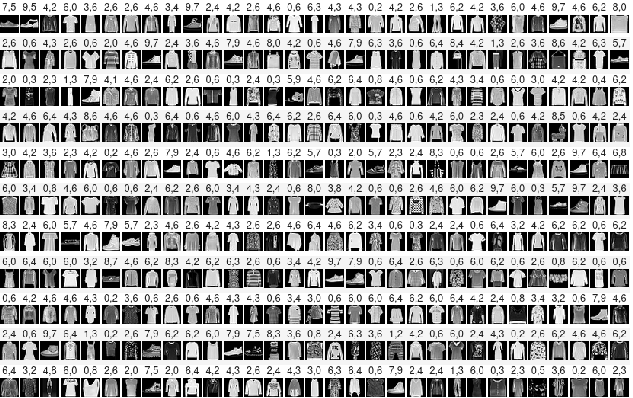
\includegraphics[width=\linewidth]{sum.png}
    \caption{Summary}
    \label{fig:Summary}
\end{figure}

% TODO If you have any insight into why it performed well, explain.
After trialing multiple variations of the network, we realized that 25 epochs often
produced the highest validation accuracy, while also minimizing loss. We further
experimented with ways of improving our accuracy by adding a dropout layer, which
we found to be effective, as well as changing our optimizer to the Adam algorithm.
Each of these steps sequentially increased our accuracy. We also found that a larger
number of filters was beneficial in increasing accuracy and thus improving performance.
Prior to adding the dropout layer and changing optimizers, we had an accuracy of
around 90%. The dropout layer and Adam algorithm were helpful in increasing our
validation accuracy and improving our overall performance, though we noticed that
our losses increased as well.


\section{Training}

% TODO Run your network from scratch at least 5 times.

% TODO Include a table showing the validation results of each of the runs
% as well as the average performance over all runs.

\begin{center}
\begin{tabular}{ |c|c|c|c|c|c|c| }
 \hline
 run number & run 1 & run 2  & run 3 & run 4 & run 5 & average \\
 val loss & 0.2514 & 0.2560 & 0.3014 & 0.2662 & 0.2715 & 0.2693 \\
 val accuracy & 0.9309 & 0.9319 & 0.9267 & 0.9307 & 0.9318 & 0.9304 \\
 \hline
\end{tabular}
\end{center}

% TODO Include a screen shot of a typical learning graphs from these runs.
\begin{figure}
    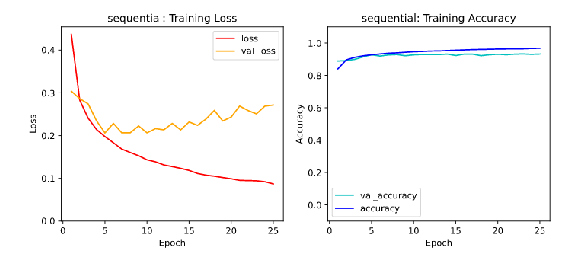
\includegraphics[width=\linewidth]{adam.png}
    \caption{training graph}
    \label{fig:training graph}
\end{figure}

\section{Evaluation}

% TODO Explain what your network was good at and why.
Our network was good at labeling shirts and dresses. They have very distinctive
shapes and their differences are simple in that they vary in terms of length,
so they are among the easiest items to label and distinguish from one another,
unlike distinguishing between a high-top sneaker and an ankle boot.
% TODO Explain what your network was bad at and why.
Our network was worst at labeling sneakers. This is likely because the images
of sneakers include different orientations, with the shoes facing both left and
right, while other clothing items have more standardized orientations and presentations.
In this way, it is difficult to generalize the image of a sneaker with our neural
network, as it presents a different challenge from the other items of clothing
we analyzed.

% TODO Include screenshots of the feature maps of convolution and/or
% pooling layers to support your analysis.
\begin{figure}
    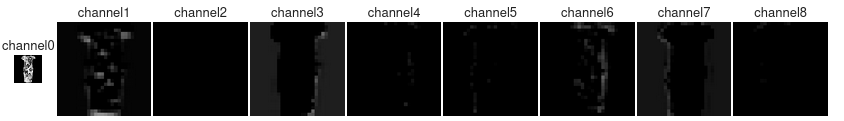
\includegraphics[width=\linewidth]{fm.png}
    \caption{Feature Map}
    \label{fig:Feature Map}
\end{figure}


\end{document}
